\documentclass[12pt,a4paper]{article}

% --- Настройка языка и шрифтов для LuaLaTeX ---
\usepackage{fontspec}
\defaultfontfeatures{Ligatures=TeX,Scale=MatchLowercase}

\setmainfont{Alice-Regular}[
    Path=font/,
    Extension=.ttf,
    BoldFont = Alice-Regular,
    ItalicFont = Alice-Regular,
    BoldItalicFont = Alice-Regular,
    BoldFeatures = {FakeBold=1.6},
    ItalicFeatures = {FakeSlant=0.2},
    BoldItalicFeatures = {FakeBold=1.6,FakeSlant=0.2}
]

\newfontfamily\cyrillicfont{Alice-Regular}[
    Path=font/,
    Extension=.ttf,
    BoldFont = Alice-Regular,
    ItalicFont = Alice-Regular,
    BoldItalicFont = Alice-Regular,
    BoldFeatures = {FakeBold=1.6},
    ItalicFeatures = {FakeSlant=0.2},
    BoldItalicFeatures = {FakeBold=1.6,FakeSlant=0.2}
]

\usepackage{polyglossia}
\setmainlanguage{russian}
\setsansfont{TeX Gyre Heros}
\setmonofont{TeX Gyre Cursor}

\usepackage{graphicx}        					          % Графика
\usepackage[protrusion=false]{microtype}       	% Микротипографика
\usepackage{amsmath, amsfonts, amssymb, amsthm}	% Математика
\usepackage{braket} 							              % Braket нотация для квантовой механики
\usepackage{unicode-math} 						          % Современный пакет для математики в LuaLaTeX
\usepackage{longtable}       					          % Таблицы с разрывом страниц
\usepackage{tikz}           					          % Рисование
\usepackage[europeanresistors]{circuitikz}		  % Рисование электрических схем в европейском стиле
\usepackage{listings}							              % Для отображения кода
\usepackage{tabularx}       					          % Для таблиц во всю ширину
\usepackage{array}		  						            % Для расширенных возможностей таблиц
\usepackage{float}          					          % Для точного позиционирования фигур
\usepackage{pgfplots}                           % Для построения графиков
\usepackage{caption}                            % Для настройки подписей к рисункам и таблицам
\usepackage{xfp}                                % Для вычислений в LaTeX
\usepackage{luacode}                            % Для выполнения Lua-кода в документе
\pgfplotsset{compat=1.18}
\usepackage[a4paper,left=20mm,right=20mm,top=20mm,bottom=20mm]{geometry}

\usetikzlibrary{arrows.meta}

% --- Колонтитулы ---
\usepackage{fancyhdr}
\pagestyle{fancy}
\fancyhf{}

\renewcommand{\headrulewidth}{0.4pt}
\renewcommand{\footrulewidth}{0.4pt}
\renewcommand\lstlistingname{Исходный код}

\lstdefinestyle{main}{
	backgroundcolor=\color{gray!8},   
	commentstyle=\color{green!50!black},
	keywordstyle=\color{blue!80!black},
	numberstyle=\small\color{darkgray},
	stringstyle=\rmfamily\color{orange!90!black},
	basicstyle=\ttfamily\small,
	breakatwhitespace=false,         
	breaklines=true,                   
	keepspaces=true,                 
	numbers=left,                    
	numbersep=8pt,                  
	showspaces=false,                
	showstringspaces=false,
	showtabs=false,                  
	tabsize=4
}	

\lstset{style=main}

\newcolumntype{C}{>{\centering\arraybackslash}X}
\renewcommand{\arraystretch}{1.25}

% =========================================================
%         СЛУЖЕБНЫЕ КОМАНДЫ ДЛЯ ВЫЧИСЛЕНИЙ
% =========================================================
\newcommand{\CalcZero} [1]{\fpeval{round((#1),0)}}
\newcommand{\CalcOne}  [1]{\fpeval{round((#1),1)}}
\newcommand{\CalcTwo}  [1]{\fpeval{round((#1),2)}}
\newcommand{\CalcThree}[1]{\fpeval{round((#1),3)}}
\newcommand{\CalcFour} [1]{\fpeval{round((#1),4)}}
\newcommand{\CalcFive} [1]{\fpeval{round((#1),5)}}

% ---------------------------------------------------------
% ОБЩИЕ ДАННЫЕ
% ---------------------------------------------------------
\def\VariantN{1}          					                   % Номер варианта
\def\StudentName{Андреев Иван Алексеевич}  	           % ФИO студента
\def\TeacherName{Журавлев Максим Николаевич}           % ФИO преподавателя
\def\LabNumber{4}							                         % Номер лабораторной работы
\def\Discipline{Квантовая механика}				             % Название дисциплины
\def\LabTitle{Движение электрона в потенциальной яме}	 % Название лабораторной работы

\begin{luacode*}

-- Константы
m = 9.1 * 10^(-31)  -- масса электрона в килограммах
h = 1.05 * 10^(-34) -- постоянная Дирака в джоулях на секунду


-- Для значения заданий 1, 2, 3 согласно варианту 
a = 2 * 10^(-10)  -- ширина ямы в метрах

-- Для заданий 4, 5 согласно варианту
U1 = 2.0  -- высота левого барьера в эВ
U2 = 3.6  -- высота правого барьера в эВ

-- Task01
E1 = 9.34 -- eV
E2 = 37.37 -- eV
E3 = 84.08 -- eV

function insertTask01()
    tex.print(" $" .. E1 .. "$ & $" .. E2 .. "$ & $" .. E3 .. "$ ")
end

-- Task03
I1 = {0.1905, 0.6039, 0.1955}
I2 = {0.3972, 0.1906, 0.4022}
I3 = {0.3333, 0.3333, 0.3333}

II = {0.9900, 0.9900, 1.0000}

function insertTask03()
    tex.print("$E_1$ & $" .. I1[1] .. "$ & $" .. I1[2] .. "$ & $" .. I1[3] .. "$ & $" .. II[1] .. "$ \\\\ \\hline")
    tex.print("$E_2$ & $" .. I2[1] .. "$ & $" .. I2[2] .. "$ & $" .. I2[3] .. "$ & $" .. II[2] .. "$ \\\\ \\hline")
    tex.print("$E_3$ & $" .. I3[1] .. "$ & $" .. I3[2] .. "$ & $" .. I3[3] .. "$ & $" .. II[3] .. "$ ")
end

-- Task04

a3 = 9.7 -- граничная ширина ямы в Ангстремах при которой ещё существует 3 уровень энергии
-- 0.2533    0.9872    1.9979
E31 = 0.2533 -- eV
E32 = 0.9872 -- eV
E33 = 1.9979 -- eV

a2 = 5.4 -- граничная ширина ямы в Ангстремах при которой ещё существует 2 уровень энергии
-- 0.5970    1.9954
E21 = 0.5970 -- eV
E22 = 1.9954 -- eV

a1 = 1.1 -- граничная ширина ямы в Ангстремах при которой ещё существует 1 уровень энергии
E11 = 1.9914 -- eV

function insertTask04()
    tex.print("$" .. a3 .. "$ & $" .. U1 .. "$ & $" .. U2 .. "$ & $" .. E31 .. "$ & $" .. E32 .. "$ & $" .. E33 .. "$ \\\\ \\hline")
    tex.print("$" .. a2 .. "$ & $" .. U1 .. "$ & $" .. U2 .. "$ & $" .. E21 .. "$ & $" .. E22 .. "$ &       — \\\\ \\hline")
    tex.print("$" .. a1 .. "$ & $" .. U1 .. "$ & $" .. U2 .. "$ & $" .. E11 .. "$ &       —         &       — ")
end

-- Task05

-- Вероятности уровней при a3

-- 0.0152    0.9786    0.0061
-- 0.0743    0.8999    0.0257
-- 0.7899    0.1942    0.0159
P311 = 0.0152
P312 = 0.9786
P313 = 0.0061

P321 = 0.0743
P322 = 0.8999
P323 = 0.0257

P331 = 0.7899
P332 = 0.1942
P333 = 0.0159

function insertTask05_1() 
    tex.print("$E_1$ & $" .. P311 .. "$ & $" .. P312 .. "$ & $" .. P313 .. "$ & $" .. P311 + P312 + P313 .. "$ \\\\ \\hline")
    tex.print("$E_2$ & $" .. P321 .. "$ & $" .. P322 .. "$ & $" .. P323 .. "$ & $" .. P321 + P322 + P323 .. "$ \\\\ \\hline")
    tex.print("$E_3$ & $" .. P331 .. "$ & $" .. P332 .. "$ & $" .. P333 .. "$ & $" .. P331 + P332 + P333 .. "$ ")
end

-- Вероятности уровней при a2

-- 0.0601    0.9171    0.0228
-- 0.8035    0.1726    0.0239

P211 = 0.0601
P212 = 0.9171
P213 = 0.0228

P221 = 0.8035
P222 = 0.1726
P223 = 0.0239

function insertTask05_2() 
    tex.print("$E_1$ & $" .. P211 .. "$ & $" .. P212 .. "$ & $" .. P213 .. "$ & $" .. P211 + P212 + P213 .. "$ \\\\ \\hline")
    tex.print("$E_2$ & $" .. P221 .. "$ & $" .. P222 .. "$ & $" .. P223 .. "$ & $" .. P221 + P222 + P223 .. "$ ")
end

-- Вероятности уровней при a1

-- 0.8846    0.0794    0.0359

P111 = 0.8846
P112 = 0.0794
P113 = 0.0359

function insertTask05_3() 
    tex.print("$E_1$ & $" .. P111 .. "$ & $" .. P112 .. "$ & $" .. P113 .. "$ & $" .. P111 + P112 + P113 .. "$ ")
end

\end{luacode*}

\title{
	МИНОБРНАУКИ РОССИИ

	федеральное государственное автономное образовательное учреждение

	высшего образования

	«Национальный исследовательский университет
	«Московский институт электронной техники»
	\vspace{2em}
}
\author{
}
\date{}

\begin{document}

\maketitle
\thispagestyle{fancy}

\begin{center}
\Large Отчёт по Лабораторной работе $\LabNumber$\\
по дисциплине «\Discipline»\\
«\LabTitle»
\end{center}

\begin{center}
\Large Вариант \VariantN
\end{center}

\vspace{12em}

\begin{table}[h]
\noindent
\begin{tabular*}{\textwidth}{@{\extracolsep{\fill}} p{0.48\textwidth} p{0.52\textwidth}}
Студент, группа & \StudentName, ЭН-$25$ \\
[0.5em] Руководитель & \TeacherName
\end{tabular*}
\end{table}

\cfoot{Москва 2026}

\pagebreak

\fancyhead[L]{\LabTitle} 
\fancyhead[R]{\Discipline}
\fancyfoot[C]{\thepage}

\section{Программа для вычисления энергитических уровней электрона в 
бесконечно-глубокой потенциальной яме}

Согласно варианту принимаем ширину потенциальной 
ямы $a = \CalcTwo{\directlua{tex.print(a * 10^10)}}$ А. Выполняем подсчёт уровней согласно формуле 
\begin{equation}
    E_n = \frac{\hbar^2 k_n^2}{2 m} \qquad k_n = \frac{n \pi}{a}
\end{equation}

\begin{lstlisting}[language=Matlab, firstnumber=12, 
	title={\textbf{Task01.m}}]
m = 9.1e-31;  %mass of electron (kg)
e = 1.6e-19;  %elementary charge (C)
h = 1.05e-34; %Plank's constant (J*s)
a = 2e-10;    %width (m)

n = [1, 2, 3];   %quantum number 

k = pi .* n ./ a; %wave number (1/m)

E = (h^2 .* k.^2) ./ (2 * m); % energy of electron (J)
\end{lstlisting}

Рисуем график в ангстремах и электронвольтах

\begin{lstlisting}[language=Matlab, firstnumber=27, 
	title={\textbf{Task01.m}}]
E = E / e;    % energy of electron (eV)
a = a * 1e10; % width in Angstroms
\end{lstlisting}

\begin{lstlisting}[language=Matlab, firstnumber=34]
fig = figure();

ax = axes(fig);
hold(ax, 'on');

grid(ax, 'on');
ax.XMinorGrid = 'on';
ax.YMinorGrid = 'on';

ax.GridAlpha = 0.55;
ax.MinorGridAlpha = 0.25;

ax.LineWidth = 0.9;
ax.Box = 'on';

ax.FontName = 'Times New Roman';
ax.FontSize = 12;

ArrowU = quiver(0, 0, 0, 100, 0, 'Color', 'black', 'LineWidth', 1.5, 'MaxHeadSize', 0.01, 'AutoScale', 'off');
ArrowX = quiver(-a * 0.5, 0, a * 2, 0, 'Color', 'black', 'LineWidth', 1.5, 'MaxHeadSize', 0.01, 'AutoScale', 'off');

Utext = text(-a * 0.2, 100 * 0.95, '$U(x)$', 'FontSize', 14, 'Color', 'black', 'VerticalAlignment', 'middle', 'HorizontalAlignment', 'left', 'Interpreter', 'latex');
Xtext = text(a * 1.5 * 0.95, -10, '$x$', 'FontSize', 14, 'Color', 'black', 'VerticalAlignment', 'bottom', 'HorizontalAlignment', 'center', 'Interpreter', 'latex');

E1 = line([0, a], [E(1), E(1)], 'Color', 'red', 'LineWidth', 2, 'DisplayName', 'E_{1}');
Etext1 = text(a * 0.5, E(1) + 0.1, '$E_{1}$', 'FontSize', 14, 'Color', 'black', 'VerticalAlignment', 'bottom', 'Interpreter', 'latex');
E2 = line([0, a], [E(2), E(2)], 'Color', 'red', 'LineWidth', 2, 'DisplayName', 'E_{2}');
Etext2 = text(a * 0.5, E(2) + 0.1, '$E_{2}$', 'FontSize', 14, 'Color', 'black', 'VerticalAlignment', 'bottom', 'Interpreter', 'latex');
E3 = line([0, a], [E(3), E(3)], 'Color', 'red', 'LineWidth', 2, 'DisplayName', 'E_{3}');
Etext3 = text(a * 0.5, E(3) + 0.1, '$E_{3}$', 'FontSize', 14, 'Color', 'black', 'VerticalAlignment', 'bottom', 'Interpreter', 'latex');

P1 = line([0, 0, a, a], [100, 0, 0, 100], 'Color', 'blue', 'LineWidth', 3, 'DisplayName', 'U(x)');

P1text = text(a * 0.55, -5, '$a$', 'FontSize', 14, 'Color', 'black', 'VerticalAlignment', 'middle', 'HorizontalAlignment', 'center', 'Interpreter', 'latex');

xlabel('$x\ (\AA)$', 'Interpreter', 'latex')
ylabel('$U(x), E\ ($eV$)$', 'Interpreter', 'latex')

title('$U(x), E$', 'Interpreter', 'latex')
\end{lstlisting}

Выводим уровни энергии в консоль
\begin{lstlisting}[language=Matlab, firstnumber=30, 
    title={\textbf{Task01.m}}]
fprintf("E1 = %.2f eV\n", E(1));
fprintf("E2 = %.2f eV\n", E(2));
fprintf("E3 = %.2f eV\n", E(3));
\end{lstlisting}

Заполним таблицу значениями уровней энергии
\begin{table}[H]
\noindent
\begin{tabularx}{\textwidth}{|C|C|C|C|}
    \hline
    $a$, \AA & \multicolumn{3}{p{10cm}|}{\centering $\CalcTwo{\directlua{tex.print(a * 10^10)}}$} \\
    \hline
    $n$ & $1$ & $2$ & $3$ \\
    \hline
    $E_n$, эВ & \directlua{insertTask01()} \\
    \hline
\end{tabularx}
\end{table}

\begin{figure}[H]
    \centering
    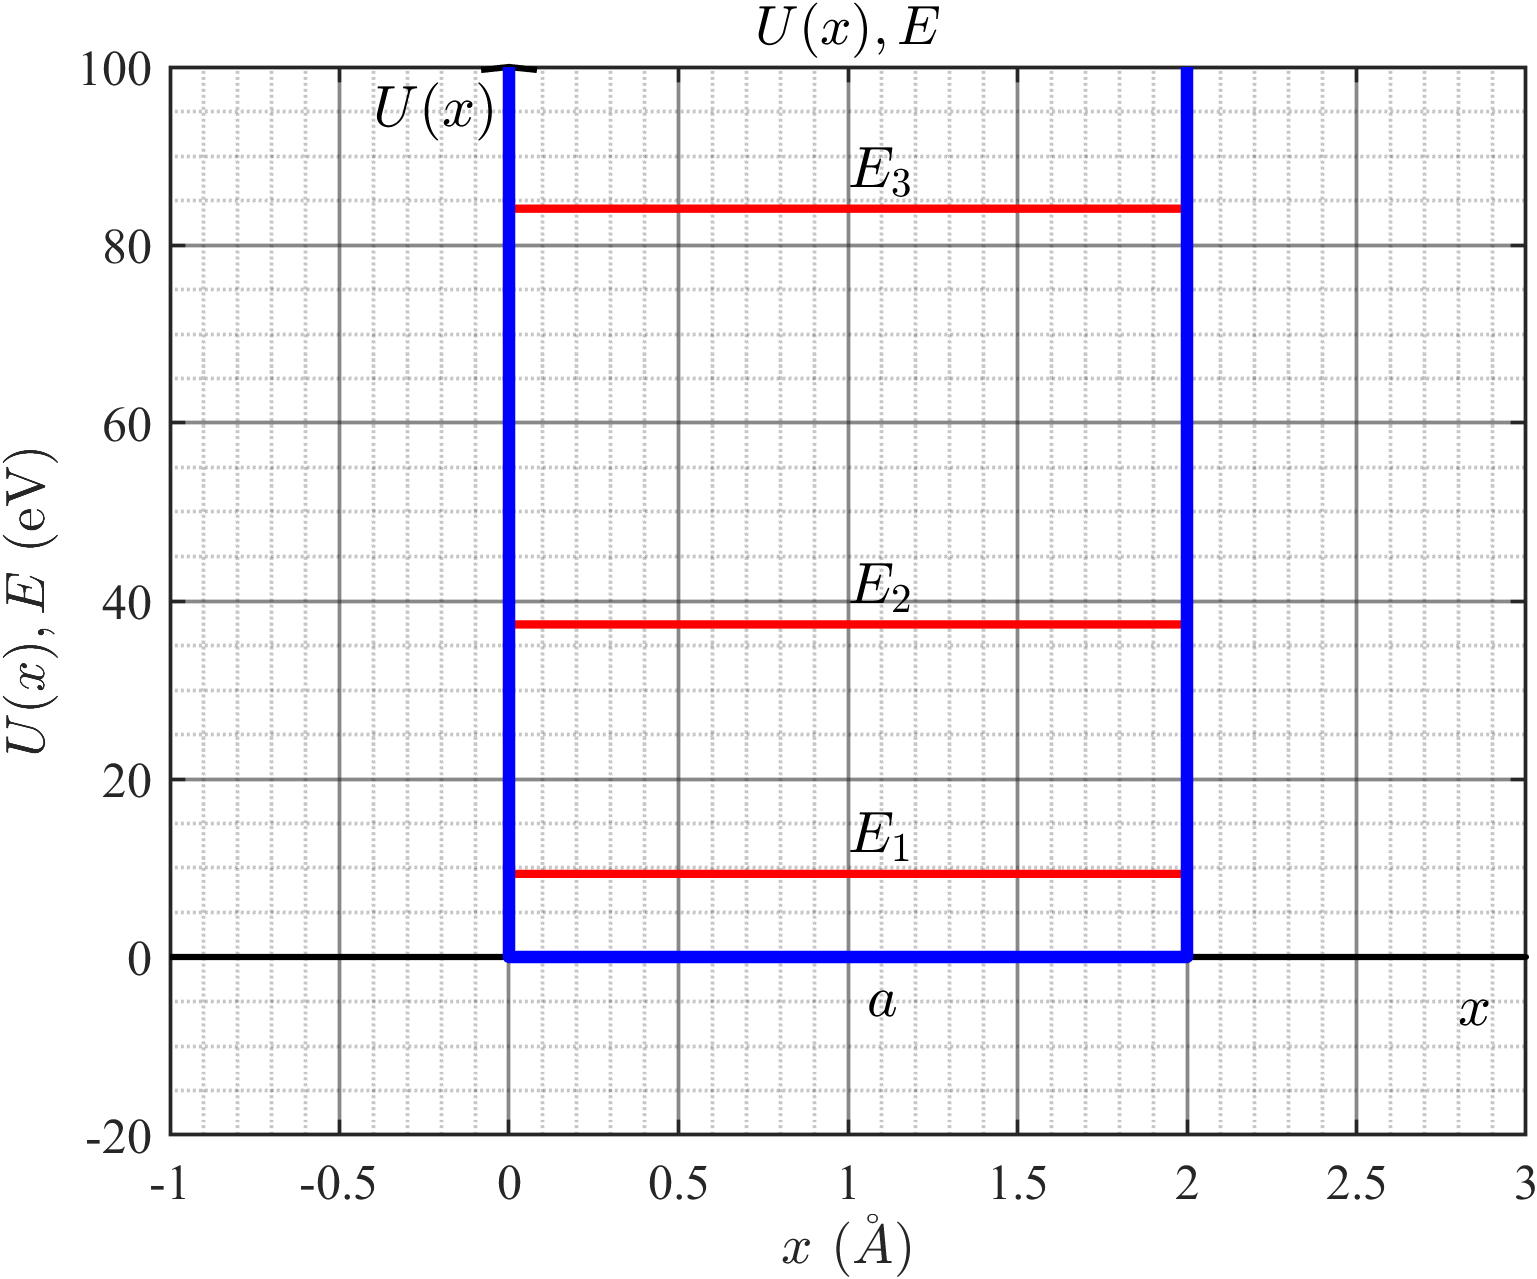
\includegraphics[width=\textwidth]{Task01/Task01.png}
    \caption{Бесконечно-глубокая потенциальная яма и уровни энергии электрона}
\end{figure}

\section{Программа для отрисовки волновых функций электрона в бесконечно-глубокой 
потенциальной яме}

Вычисляем волновые функции для трёх первых уровней энергии
\begin{equation}
    \psi_n(x) = \sqrt{\frac{2}{a}} \sin\left(\frac{n \pi x}{a}\right)
\end{equation}

\begin{lstlisting}[language=Matlab, firstnumber=12, 
    title={\textbf{Task02.m}}]
m = 9.1e-31;  %mass of electron (kg)
h = 1.05e-34; %Plank's constant (J*s)
a = 2;        %width of potential well (Angstroms)

x = 0:0.01:a; %x in Angstroms

n = [1, 2, 3];   %quantum number

psi = @(n, x) sqrt(2 / a) * sin(n * pi * x / a); %wave function

psi1 = psi(n(1), x);
psi2 = psi(n(2), x);
psi3 = psi(n(3), x);
\end{lstlisting}

Рисуем график в ангстремах

\begin{lstlisting}[language=Matlab, firstnumber=26, 
    title={\textbf{Task02.m}}]
fig = figure();

ax = axes(fig);
hold(ax, 'on');

grid(ax, 'on');
ax.XMinorGrid = 'on';
ax.YMinorGrid = 'on';

ax.GridAlpha = 0.55;
ax.MinorGridAlpha = 0.25;

ax.LineWidth = 0.9;
ax.Box = 'on';

ax.FontName = 'Times New Roman';
ax.FontSize = 12;

ArrowPsi = quiver(0, 0, 0, 1.5, 0, 'Color', 'black', 'LineWidth', 1.5, 'MaxHeadSize', 0.3, 'AutoScale', 'off');
ArrowX = quiver(-a * 0.5, 0, a * 2, 0, 'Color', 'black', 'LineWidth', 1.5, 'MaxHeadSize', 0.1, 'AutoScale', 'off');

Utext = text(-a * 0.2, 1.5 * 0.9, '$\Psi(x)$', 'FontSize', 14, 'Color', 'black', 'VerticalAlignment', 'middle', 'HorizontalAlignment', 'left', 'Interpreter', 'latex');
Xtext = text(a * 1.5 * 0.95, -0.2, '$x$', 'FontSize', 14, 'Color', 'black', 'VerticalAlignment', 'bottom', 'HorizontalAlignment', 'center', 'Interpreter', 'latex');

Psi1 = plot(x, psi1, 'Color', 'red', 'LineWidth', 2, 'DisplayName', '$\Psi_{1}$');
Psitext1 = text(a * 0.5, 1, '$\Psi_{1}$', 'FontSize', 14, 'Color', 'black', 'VerticalAlignment', 'bottom', 'Interpreter', 'latex');
Psi2 = plot(x, psi2, 'Color', 'red', 'LineWidth', 2, 'DisplayName', '$\Psi_{2}$');
Psitext2 = text(a * 0.45, -1.2, '$\Psi_{2}$', 'FontSize', 14, 'Color', 'black', 'VerticalAlignment', 'bottom', 'Interpreter', 'latex');
Psi3 = plot(x, psi3, 'Color', 'red', 'LineWidth', 2, 'DisplayName', '$\Psi_{3}$');
Psitext3 = text(a * 0.7, -1.2, '$\Psi_{3}$', 'FontSize', 14, 'Color', 'black', 'VerticalAlignment', 'bottom', 'Interpreter', 'latex');

P1 = line([0, 0], [-1.5, 1.5], 'Color', 'blue', 'LineWidth', 3);
P2 = line([a, a], [-1.5, 1.5], 'Color', 'blue', 'LineWidth', 3);

P1text = text(a * 1.05, -0.1, '$a$', 'FontSize', 14, 'Color', 'black', 'VerticalAlignment', 'middle', 'HorizontalAlignment', 'center', 'Interpreter', 'latex');

xlabel('$x\ (\AA)$', 'Interpreter', 'latex')
ylabel('$\Psi(x)\ (\AA^{-1/2})$', 'Interpreter', 'latex')

title('$\Psi(x)$', 'Interpreter', 'latex')
\end{lstlisting}

\begin{figure}[H]
    \centering
    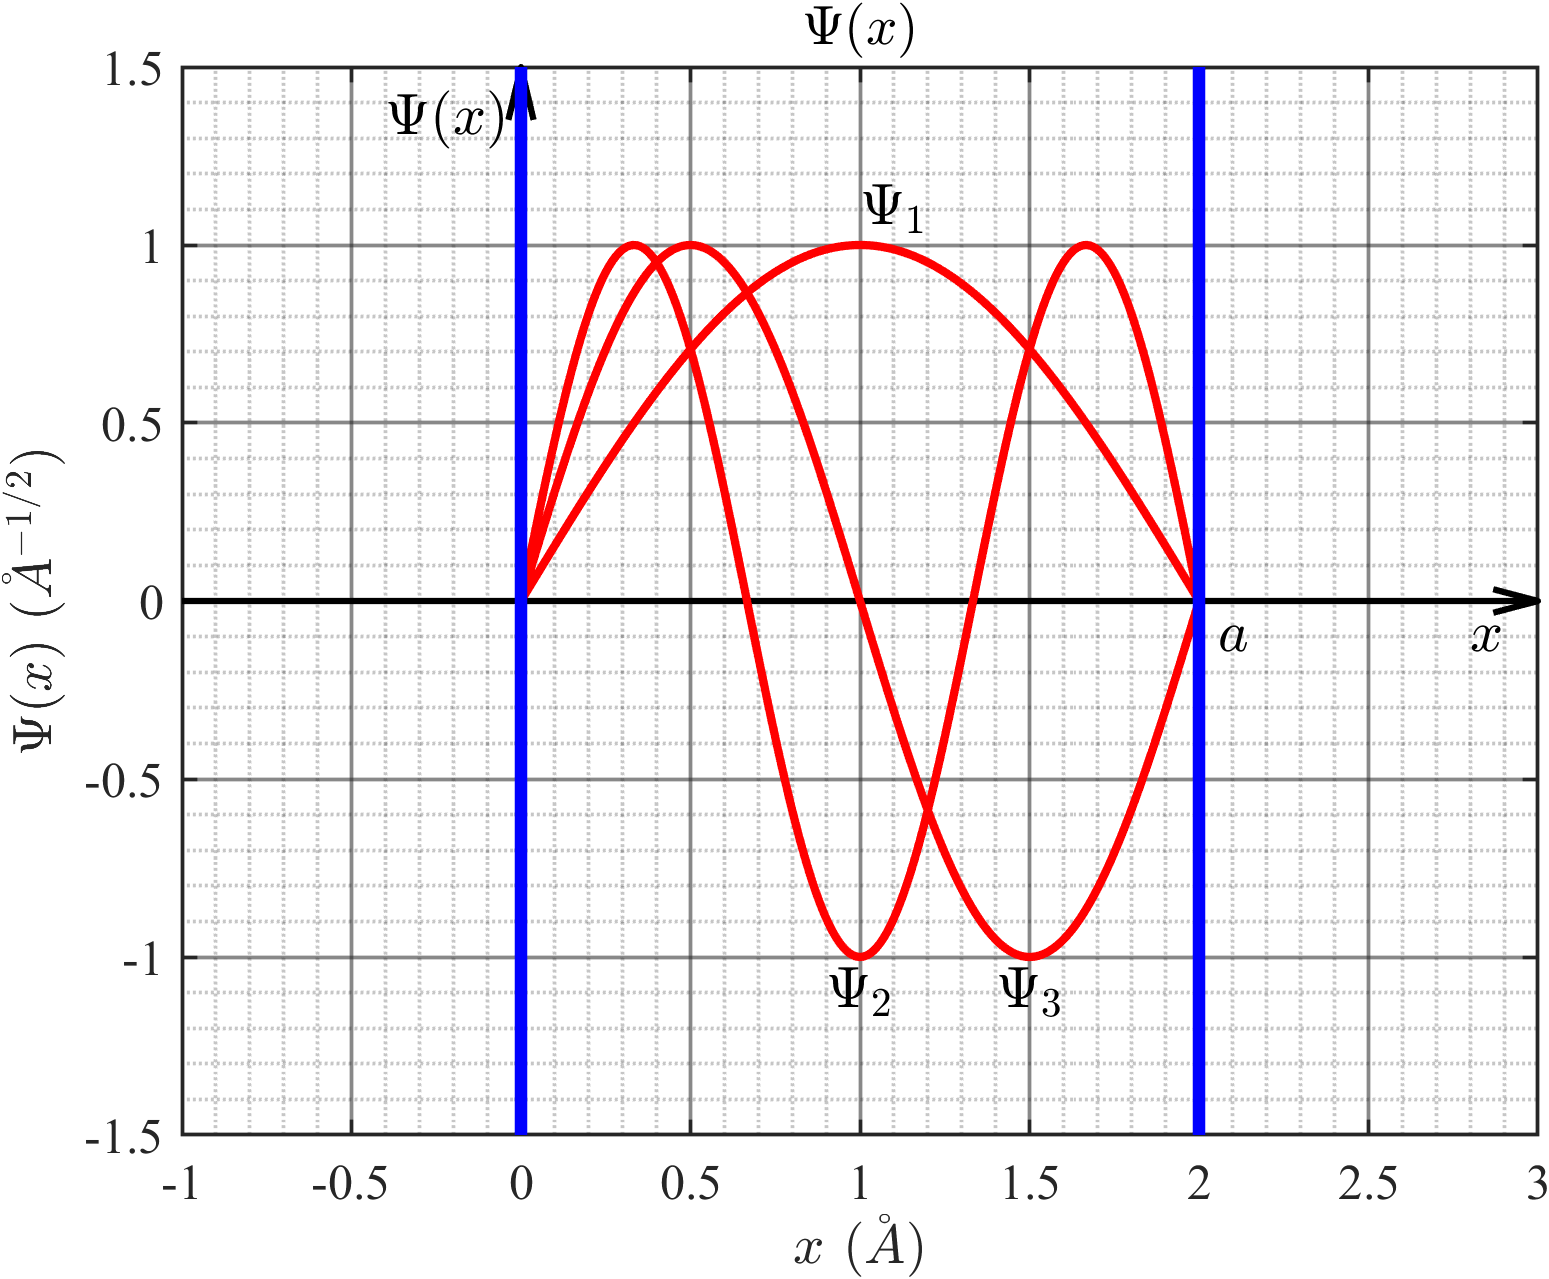
\includegraphics[width=\textwidth]{Task02/Task02.png}
    \caption{Бесконечно-глубокая потенциальная яма и волновые функции электрона}
\end{figure}

\section{Программа для подсчёта вероятности нахождения электрона в области 
бесконечно-глубокой потенциальной ямы}

Используем функцию численного вычисления интегралов для подсчёта вероятности найти 
электрон в различных областях потенциальной ямы и выводим результаты в консоль
\begin{equation}
    P(x_1 < x < x_2) = \frac{2}{a} \int\limits_{x_1}^{x_2} \sin^2\left(\frac{n \pi x}{a}\right) dx
\end{equation}

\begin{lstlisting}[language=Matlab, firstnumber=12, 
    title={\textbf{Task03.m}}]
m = 9.1e-31;                %mass of electron (kg)
h = 1.05e-34;               %Plank's constant (J*s)
a = 2.0;                    %width of potential well (A, Angstroem)

x1 = 0:0.01:a/3; %x in Angstroms
x2 = a/3:0.01:2*a/3;
x3 = 2*a/3:0.01:a;

n = [1, 2, 3];   %quantum number

I1 = zeros(size(n));
I2 = zeros(size(n));
I3 = zeros(size(n));

Density = @(n, x) (sqrt(2/a) * sin(n * pi * x / a)).^2;

for i = 1:length(n)
	I1(i) = trapz(x1, Density(n(i), x1));
	fprintf("Probability from 0 to a/3 for n = %d: %.4f\n", n(i), I1(i));
	I2(i) = trapz(x2, Density(n(i), x2));
	fprintf("Probability from a/3 to 2*a/3 for n = %d: %.4f\n", n(i), I2(i));
	I3(i) = trapz(x3, Density(n(i), x3));
	fprintf("Probability from 2*a/3 to a for n = %d: %.4f\n", n(i), I3(i));
end

fprintf("Sum of probabilities for n = 1: %.4f\n", I1(1) + I2(1) + I3(1));
fprintf("Sum of probabilities for n = 2: %.4f\n", I1(2) + I2(2) + I3(2));
fprintf("Sum of probabilities for n = 3: %.4f\n", I1(3) + I2(3) + I3(3));
\end{lstlisting}

Заполним таблицу значениями вероятностей нахождения электрона в различных областях ямы 
для трёх первых уровней энергии
\begin{table}[H]
    \noindent
    \centering
    \begin{tabularx}{\textwidth}{|C|C|C|C|C|}
        \hline
        & \small $P(0 < x < \frac{a}{3})$ & \small $P(\frac{a}{3} < x < \frac{2a}{3})$ & \small $P(\frac{2a}{3} < x < a)$ & $\sum P$ \\
        \hline
        \directlua{insertTask03()} \\
        \hline
    \end{tabularx}
\end{table}

\section{Исследование уровней энергии несимметричной потенциальной ямы конечной глубины}

Заданы согласно варианту высота левого барьера 
$U_1 = \CalcTwo{\directlua{tex.print(U1)}}$ эВ и высота правого барьера 
$U_2 = \CalcTwo{\directlua{tex.print(U2)}}$ эВ.

\begin{lstlisting}[language=Matlab, firstnumber=22, 
    title={\textbf{Task04.m}}]
U1 = 2.0;                  %left barier of potential well (eV)
U2 = 3.6;                  %rigth barier of potential well (eV)
\end{lstlisting}

Ищем граничные значения ширины ямы, при которых ещё существует $3$, $2$ и $1$ уровень энергии соответственно,
вносим результаты в таблицу
\begin{table}[H]
    \noindent
    \centering
    \begin{tabularx}{\textwidth}{|C|C|C|C|C|C|}
        \hline
        $a$, \AA & $U_1$, эВ & $U_2$, эВ & $E_1$, эВ & $E_2$, эВ & $E_3$, эВ \\
        \hline
        \directlua{insertTask04()} \\
        \hline
    \end{tabularx}
    \caption{Граничные ширины ямы и уровни энергии для несимметричной потенциальной ямы конечной глубины}
    \label{tab:task04}
\end{table}

\section{Численная оценка вероятности координаты электрона относительно потенциальной ямы
при граничной ширине несимметричной ямы конечной глубины}

Вносим данные в параметры программы из таблицы \ref{tab:task04}, берём данные из консоли, 
заполняем таблицу

\begin{table}[H]
    \noindent
    \centering
    \begin{tabularx}{\textwidth}{|C|C|C|C|C|}
        \hline
        & \small $P(-\infty < x < 0)$ & \small $P(0 < x < a)$ & \small $P(a < x < +\infty)$ & $\sum P$ \\
        \hline
        \directlua{insertTask05_1()} \\
        \hline
    \end{tabularx}
\end{table}

Усекаем вектор энергии в коде до двух членов и вносим данные, заполняем таблицу

\begin{table}[H]
    \noindent
    \centering
    \begin{tabularx}{\textwidth}{|C|C|C|C|C|}
        \hline
        & \small $P(-\infty < x < 0)$ & \small $P(0 < x < a)$ & \small $P(a < x < +\infty)$ & $\sum P$ \\
        \hline
        \directlua{insertTask05_2()} \\
        \hline
    \end{tabularx}
\end{table}

Усекаем вектор энергии в коде до одного члена и вносим данные, заполняем таблицу

\begin{table}[H]
    \noindent
    \centering
    \begin{tabularx}{\textwidth}{|C|C|C|C|C|}
        \hline
        & \small $P(-\infty < x < 0)$ & \small $P(0 < x < a)$ & \small $P(a < x < +\infty)$ & $\sum P$ \\
        \hline
        \directlua{insertTask05_3()} \\
        \hline
    \end{tabularx}
\end{table}

\end{document}